%% LyX 2.3.2-2 created this file.  For more info, see http://www.lyx.org/.
%% Do not edit unless you really know what you are doing.
\documentclass[english]{IEEEtran}
\usepackage[T1]{fontenc}
\usepackage[latin9]{inputenc}
\usepackage{array}
\usepackage{float}
\usepackage{multirow}
\usepackage{amsmath}
\usepackage{graphicx}

\makeatletter

%%%%%%%%%%%%%%%%%%%%%%%%%%%%%% LyX specific LaTeX commands.
\newcommand{\lyxmathsym}[1]{\ifmmode\begingroup\def\b@ld{bold}
  \text{\ifx\math@version\b@ld\bfseries\fi#1}\endgroup\else#1\fi}

%% Because html converters don't know tabularnewline
\providecommand{\tabularnewline}{\\}

\makeatother

\usepackage{babel}
\begin{document}
\title{An effecient automatic segmentation of left ventricle by hybrid approach}
\author{\IEEEauthorblockN{M. Arsalan KHAWAJA\IEEEauthorrefmark{1} and Bui Thien Bao\IEEEauthorrefmark{2}\\
} \IEEEauthorblockA{\IEEEauthorrefmark{1}Center Universitaire Condorcet,\\
Universite de Bourgogne,\\
71200, Le Creusot,\\
France.\\
Email : Muhammad-Arsalan\_Khawaja@etu.u-bourgogne.fr\\
}\IEEEauthorblockA{\IEEEauthorrefmark{2}Center Universitaire Condorcet,\\
Universite de Bourgogne,\\
71200, Le Creusot,\\
France.\\
Email :}}
\maketitle
\begin{abstract}
Left Ventricle is an integral part of the heart. It pumps blood into
the body. Cardiovascular diseaes are quite common in modern world.
The health of the heart can be studied using left ventricle. Most
of the heart diseases can be diagnosed by retrieving important information
from systole and diastole operations of heart via effective medical
imaging analysis of Left Ventricle (LV). The segmentation of Left
Ventricle plays an important role in retrieving the ejection fraction
(a parameter which indicates the heart's health). Since Magnetic Resonance
Images (MRI) are noisy and not really perfect, scientific community
is always curious to find more effecient, reliable, robust and more
accurate segmentation methods to calculate ejection fraction. In this
research project, we use a novel hybrid approach for segmentation.
K-means, along with border following algorithm is used for segmentation.
The results are quite impressive and discussed in the last section.
\end{abstract}

\begin{IEEEkeywords}
K-means, Python, Border Following Algorithm, Left Ventricle, Adaptive
Smoothing, Clustering, Hough Transform.
\end{IEEEkeywords}


\section{Introduction}

The segmentation of left ventricle is of utmost importance when it
come to diagnosis of heart diseases. It takes too much of a time for
manual segmentation and is a painstaking task. This segmentation establishes
and provides us with important knowledge of critical parameters which
can help us calculate certain ratios. These ratios help doctors to
predict the condition of heart and in some cases diagnose a particular
disease. In short, an efficeint segmentation of heart ends up saving
patient life.

Unfortunately doctors are too busy to manually segment each of the
medical image and it also wastes alot of thier time. They are more
needed to patients. There is an inevitable demand for some automatic
segmentation of left ventricle. Alot of work has been done in this
field, but because medical images are not really the most perfect
images, segmentation algorithms are destined to struggle with accuracy.
Some of the most common methods used for demonstrated in figure \ref{fig:These-are-some}.

\begin{figure}[H]

\begin{centering}
\includegraphics[scale=0.7]{\string"methodsfor LVseg\string".PNG}\caption{\label{fig:These-are-some}These are some methods / Algorithms used
to segment left ventricle. Each of them have their own advantages
and disadvatages. None of them is perfect.}
\par\end{centering}
\end{figure}

We went through the algorithms and decided to use Hybrid Appoach for
our segmentation. In hybrid approach, we intend to use more than one
approaches / algorithms to work simaltaneosly on the segmentation
of the image. In this project we used mainly primarily K-Means algorithm
inspired by \cite{lynch2006automatic}. Alongside, a border following
algorithm inspired from \cite{suzuki1985topological} was used to
enhance segmentation results. The preproccessing was done with adaptive
smoothing algorithm. Finally we optimized the performance of our algorithm
by repeated experiments of using the algorithm with different datasets
and setting the parameters to optimal value.

\section{Anatomy of Heart}

The heart is made up of four chambers: two upper chambers known as
the left atrium and right atrium and two lower chambers called the
left and right ventricles. These are shown in following figure .

\begin{figure}[H]

\centering{}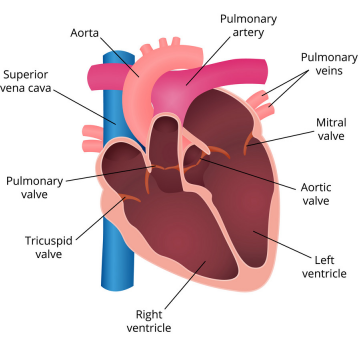
\includegraphics[scale=0.6]{heart.PNG}\caption{The left ventricle is longer and more conical in shape. In short axis,
the left ventricle appears circular in shape. The image is taken from
\cite{websiteforimageheart}}
\end{figure}
The left ventricle is considered an important part of the cardiovascular
system. It is thought off as a pump that supplies blood to the body.
The mass of the left ventricle, as estimated by magnetic resonance
imaging, averages $143g\pm38.4g$, with a range of $87\lyxmathsym{\textendash}224g$
\cite{coogan2013computational}.

Another important thing to discuss are the two phases of the cardiac
cycle. They are called Systole and Diastole. They occur as the heart
beats, pumping blood through a system of blood vessels that carry
blood to every part of the body. Systole occurs when the heart contracts
to pump blood out, and diastole occurs when the heart relaxes after
contraction.

\subsection{Ejection Fraction}

Ejection fraction (EF) refers to how well your left ventricle (or
right ventricle) pumps blood with each heart beat \cite{lynch2006automatic}.
The ejection fraction can be calculated as follows:

\begin{equation}
\mathrm{EF}=\frac{V_{\mathrm{endo}}\left(t_{\mathrm{D}}\right)-V_{\mathrm{endo}}(t\mathrm{s})}{V_{\mathrm{endo}}\left(t_{\mathrm{D}}\right)}\label{eq:-9}
\end{equation}

Here note that $V_{endo}$ is the volume of the inner walls of the
heart, $V_{endo}(t_{D})=max_{t}[V_{endo}(t)]$ is the end-diastolic
volume and$V_{endo}(t_{S})=min_{t}[V_{endo}(t)]$ is the end-systolic
volume.

\section{Methodology}

The first task was to identify the tasks in the project. After we
were done with identifying the tasks, we came to their implementation
on python. We studied and learned to use the needed libraries in python.
The libraries hae been given in Appendix A. The following flowchart
gives a very articulate work flow \ref{fig:The-flowchart-demonstrates}
demonstration.

\begin{figure}[H]

\begin{centering}
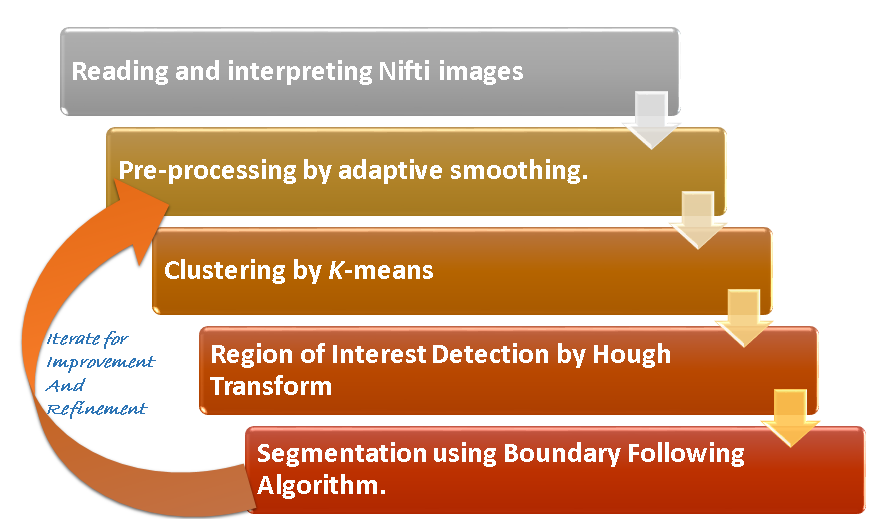
\includegraphics[scale=0.375]{methodology.PNG}\caption{\label{fig:The-flowchart-demonstrates}The flowchart demonstrates
work flow. Neccessary iterations were done to find the optimal combination
of all algorithm parameters with the goal of acheiving the highest
accuracy possible.}
\par\end{centering}
\end{figure}


\section{Development}

In this section we will discuss the implementation of algorithm. Python
programming language was used for the implementation. The methodology
from figure \ref{fig:The-flowchart-demonstrates} was observed to
complete the project. We faced challenges in almost every stage but
our resiliance and motivation kept us going. The following subsections
take us step by step through the ladder of project.

\subsection{Adaptive non linear smoothing}

We considered Feature-Preserving Adaptive Smoothing Method (FPASM)
for our project. The primary K-Means research \cite{lynch2006automatic}
that we were following took this algorithm from another research \cite{chen1999feature}.
Adaptive smoothing is a class of typical nonlinear smoothing techniques
that has been studied for many years.

The idea is to adapt pixel intensities to the local attributes of
an image on the basis of discontinuity measures. Note that in this
algorithm there are two kind of discontinuities, Local and Contextual
discontinuity. This novel approach joins these both discontinuities
to preserve edges and at same time smooths images. It is brilliant
method according to us.

In order to measure local discontinuities, we define four detectors
for pixel $(x,y)$ along four directions. These four directions are
vertical (V), horizontal (H), diagonal (D), and counter-diagonal (C),
respectively. Accordingly, four detectors are defined as \cite{chen1999feature}

\begin{equation}
\begin{array}{c}
E_{H_{xy}}=\left|I_{x+1,y}-I_{x-1,y}\right|\\
E_{V_{xy}}=\left|I_{x,y+1}-I_{x,y-1}\right|\\
E_{C_{xy}}=\left|I_{x+1,y+1}-I_{x-1,y-1}\right|\\
E_{D_{xy}}=\left|I_{x+1,y-1}-I_{x-1,y+1}\right|
\end{array}\label{eq:}
\end{equation}

Here $I_{(x,y)}$ is the intensity of pixel $(x,y)$. To be more clear
we constructed this figure \ref{fig:The-pixel-}.

\begin{figure}[H]

\begin{centering}
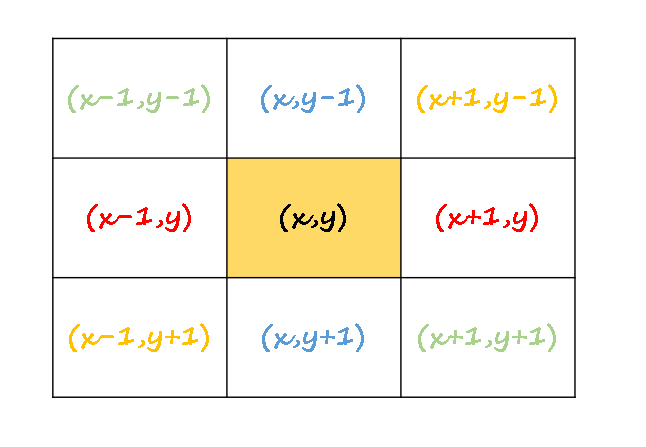
\includegraphics[scale=0.5]{localdisc}\caption{\label{fig:The-pixel-}The pixel $(x,y)$ is our pixel of operation.
We see the local discontinuity defined in equations \ref{eq:-1}\ref{eq:}
is nothing but calculating the differences around the neighbouring
pixels.}
\par\end{centering}
\end{figure}

With these diferences in mind, we define the local discontinuity as
\cite{chen1999feature}:

\begin{equation}
E_{xy}=\frac{E_{H_{xy}}+E_{V_{xy}}+E_{C_{xy}}+E_{D_{xy}}}{4}\label{eq:-1}
\end{equation}

In order to detect contextual discontinuities, we use spatial variance
to make a measure. First, we define a contextual neighborhood associated
with pixel $(x;y)$, $Nxy(R),$as \cite{chen1999feature}:

\begin{equation}
N_{xy}(R)=\{(i,j)|x-R\leq i\leq x+R,y-R\leq j\leq y+R\}\label{eq:-2}
\end{equation}

Note that, here $R(R>1)$ is a parameter that determines the size
of this contextual neighborhood. The contextual neighborhood is defined
here without explicitly counting image boundaries. The parameter $R$
describes a spatial scale or a resolution that critically determines
results of the contextual discontinuity measure. We calculate the
mean of pixels on $N_{xy}(R)$, $\mu_{xy}(R)$, as \cite{chen1999feature}:

\begin{equation}
\mu_{xy}(R)=\frac{\sum_{(i,j)\in N_{xy}(R)}I_{i,j}}{\left|N_{xy}(R)\right|}\label{eq:-3}
\end{equation}

and the spatial variance, $\sigma_{xy}^{2}(R)$, can be calculated
as \cite{chen1999feature}:

\begin{equation}
\begin{aligned}\sigma_{xy}^{2}(R) & =\frac{\sum_{(i,j)\in N_{xy}(R)}\left(I_{i,j}-\mu_{ij}(R)\right)^{2}}{\left|N_{xy}(R)\right|}\\
 & =\frac{\sum_{(i,j)\in N_{xy}(R)}I_{i,j}^{2}}{\left|N_{xy}(R)\right|}-\left(\frac{\sum_{(i,j)\in N_{xy}(R)}I_{i,j}}{\left|N_{xy}(R)\right|}\right)^{2}
\end{aligned}
\label{eq:-4}
\end{equation}

The normalized $\tilde{\sigma}_{xy}^{2}(R)$ can be written as \cite{chen1999feature}:

\begin{equation}
\tilde{\sigma}_{xy}^{2}(R)=\frac{\sigma_{xy}^{2}(R)-\sigma_{\min}^{2}(R)}{\sigma_{\max}^{2}(R)-\sigma_{\min}^{2}(R)}\label{eq:-5}
\end{equation}

where$\sigma_{\max}^{2}(R)$and $\sigma_{\min}^{2}(R)$are the maximal
and minimal spatial variance across the entire image, respectively.
Intuitively, $\tilde{\sigma}_{xy}^{2}(R)$ reflects the relative degree
of the contextual discontinuities for pixel $(x;y)$. The table \ref{tab:Interpretation-of-Spatial}
describes the influence of $\tilde{\sigma}_{xy}^{2}(R)$ in a more
articulate way on the smoothing.

\begin{table}[H]

\begin{centering}
\begin{tabular}{|c|c|c|}
Parameter & Value set & \textbf{Indication}\tabularnewline
\hline 
\multirow{4}{*}{$\boldsymbol{\tilde{\sigma}_{xy}^{2}(R)}$} & Large Value & presence of significant feature\tabularnewline
\cline{2-3} \cline{3-3} 
 & Small Value & No significant feature or significant edges found\tabularnewline
\cline{2-3} \cline{3-3} 
 & < $\theta_{\sigma}$ & usually it means noise\tabularnewline
\cline{2-3} \cline{3-3} 
 & >$\theta_{\sigma}$ & it\textquoteright s a feature\tabularnewline
\hline 
\multirow{3}{*}{$\alpha$} & Small value & fast smoothing and discontinuity reduction\tabularnewline
\cline{2-3} \cline{3-3} 
 & \multirow{2}{*}{Large value} & slow smoothing \tabularnewline
 &  & so that important features can be preserved\tabularnewline
\hline 
\multirow{2}{*}{$S$} & Small value & leads to better preservation of details\tabularnewline
\cline{2-3} \cline{3-3} 
 & Large value & all discontinuities disappear\tabularnewline
\end{tabular}\caption{\label{tab:Interpretation-of-Spatial}Analysis of changing smoothing
Parameters}
\par\end{centering}
\end{table}
So, these results reccomend us that the local attributes of a pixel
with a high contextual discontinuity should be preserved and those
of a pixel with a low contextual discontinuity should be smoothed
toward homogeneity. However, both noise and trivial features irrelevant
to a given problem lead to the complexity for visual information processing.
In order to reduce their influence in the contextual discontinuity
estimation, we introduce a transformation into $\tilde{\sigma}_{xy}^{2}(R)$\cite{chen1999feature};

\begin{equation}
\Phi\left(\tilde{\sigma}_{xy}^{2}(R),\theta_{\sigma}\right)=\left\{ \begin{array}{ll}
0 & \tilde{\sigma}_{xy}^{2}(R)<\theta_{\sigma}\\
\tilde{\sigma}_{xy}^{2}(R) & \tilde{\sigma}_{xy}^{2}(R)\geq\theta_{\sigma}
\end{array}\right.\label{eq:-6}
\end{equation}

Here $\theta_{\sigma}\left(0\leq\theta_{\sigma}\leq1\right)$ is a
threshold. For a given $\theta_{\sigma},\Phi\left(\tilde{\sigma}_{\pi v}^{2}(R),\theta_{\sigma}\right)$
gives us lead to contextual discontinuity map.In summary, pixels of
same area or region are supposed to have low contextual discontinuities
except the case, for those pixels located near boundaries that have
high contextual discontinuities. Unlike local discontinuity measure,
conextual discontinuity measure is relatively insensitive to local
intensity changes.

Now that we have established the concepts of Local Discontinuity and
Contextual discontinuity, It is easier to understand the smoothing
algorithm. The key concept of adaptive smoothing is to update a pixel\textquoteright s
intensity through the influence of local weighted averaging of its
neighboring pixels\textquoteright{} intensities. The flow chart in
figure \ref{fig:Flow-Chart-for} gives the birds eye view of smoothing
algorithm.

\begin{figure}[H]

\begin{centering}
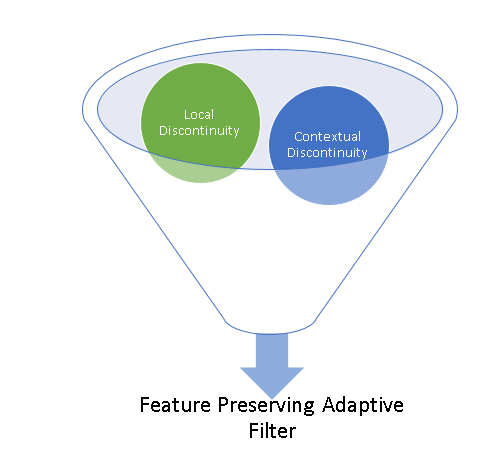
\includegraphics[scale=0.65]{funneldiagramforadaptivefilter.PNG}\caption{\label{fig:Flow-Chart-for}Flow Chart for the idea of Adaptive filter.
In step-1, we calculate local discontnuity. In step-2, we calculate
contextual discontinuity. In step-3 with the suitable guess of parameters
$R$ and $\theta$ , we use equation \ref{eq:-7} to calculate filtered
image. If the results are not satisfactory, we play with the parameters
and reclculate the filtered image upto reasonable nunmber of iterations.}
\par\end{centering}
\end{figure}

The smoothing algorithm as shown in equation \ref{eq:-7} runs through
the entire image updating each pixels intensity value $I_{xy}^{t}$,
where t is the iteration value \cite{chen1999feature}.

\begin{equation}
I_{xy}^{t+1}=I_{xy}^{t}+\eta_{xy}\frac{\Sigma_{(i,j)\in N_{xy}(1)/[(x,y)]}\eta_{ij}y_{ij}^{t}\left(I_{i,j}^{t}-I_{x,y}^{t}\right)}{\Sigma_{(i,j)\in N_{xy}(1)/[(x,y)\}}\eta_{ij}\gamma_{ij}^{t}}\label{eq:-7}
\end{equation}

here note that $\alpha$ is a parameter whose value we set according
to table \ref{tab:Interpretation-of-Spatial}:

\begin{equation}
\begin{array}{l}
\eta_{ij}=\exp\left(-\alpha\not\nabla\left(\tilde{\sigma}_{xy}^{2}(R),\theta_{\sigma}\right)\right)\\
\gamma_{ij}^{t}=\exp\left(-E_{ij}^{t}/S\right)
\end{array}\label{eq:-8}
\end{equation}

The main goal of smoothing is to alleviate the complexity for subsequent
processes in early vision. With this pre- processing, the results
of our MRI image are shown in figure \ref{fig:On-the-left,}.

\begin{figure}[H]

\begin{centering}
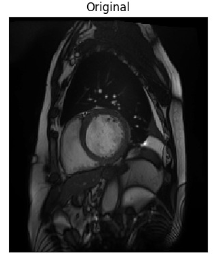
\includegraphics[scale=0.75]{original.PNG}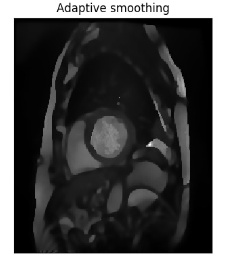
\includegraphics[scale=0.75]{AdaptiveSmoothing.PNG}\caption{\label{fig:On-the-left,}On the left, is the original image. On the
right is the smoothed image. We can clearly notice that the algorithm
has blurred the details of object but takes care of the edges. This
will help us in getting great accuracy for segmentation.}
\par\end{centering}
\end{figure}


\subsection{K-Means Clustering}

The smoothed images were then clustered using $k$-means algorithm
proposed by Duda and Hart \cite{hartigan1979algorithm,duda1973pattern}.
This algorithm has four steps as shown in figure \ref{fig:The-figure-demonstrates}
to search for the image clusters.

\begin{figure}[H]

\begin{centering}
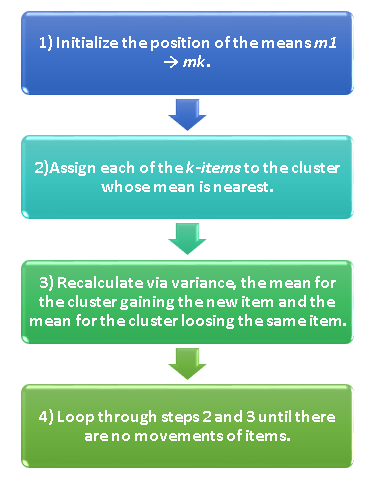
\includegraphics[scale=0.65]{flowchartforkmeans.PNG}\caption{\label{fig:The-figure-demonstrates}The figure demonstrates the process
of K-Means algorithm step by step. The algorithm is quite simple and
is widely used in Machine learning, Econmics, Data science and many
other fields.}
\par\end{centering}
\end{figure}

The key idea of the $K$ -means algorithm is to divide $M$ points
in $N$ dimensions into $K$ clusters, such that the within-cluster
sum of squares is minimized \cite{hartigan1979algorithm} .K-means
Clustering is categorized as unsupervised learning, which means that
it does not need any intervention by human in our project and leads
way to automatic segmentation of Left Ventricle. The figure \ref{fig:Clustering-of-the}
shows results after applying k-means clustering.

\begin{figure}[H]

\begin{centering}
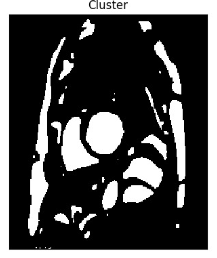
\includegraphics[scale=0.8]{clustering.PNG}\caption{\label{fig:Clustering-of-the}Clustering of the original image as
shown in figure \ref{fig:On-the-left,}. The image has been clustered
using K means algorithm with $k=2$, where $k$ is the number of clusters.}
\par\end{centering}
\end{figure}


\subsection{Detection of Region of Interest (ROI)}

It was a trickiest part of the project. We tried a number of approaches
to detect the region of interest, i.e the region containing left ventricle
and its nearby surroundings. The approaches have been defined described
briefly:

\subsubsection{Hough Transform}

We know that the left ventricle can thought of as an approximation
of circle. Hough transform is used to detect circular features in
an image. We applied hough transform and detected ventricle. With
the centre of ventricle detected as centre of circle, we declared
the reasonable area around centre of circle as region of interest.
However this approach was not a great idea because:
\begin{itemize}
\item Left ventricle is the only circular shape object in image, Many slices
had more than one circular object other than left ventricle which
allowed it hough transform to detect false left ventricle.
\item In some images / slices, left ventricle becomes too dark to be detected
as an object.
\item In some images / slices, the left ventricle is not near to circular
shape. so hough transform fails
\end{itemize}

\subsection{Segmentation of Left Ventricle}

A border following algorithm inspired by \cite{suzuki1985topological}
was used to segment Left Ventricle. Border following is one of the
most important and popular technique in segmentation of binary images.
. It derives a sequence of the coordinates or the chain codes from
the border between a connected component of l-pixels\footnote{Pixels with densities 1 are called the 1-pixel}
(l-component) and a connected component of O-pixels\footnote{Pixels with densities 0 are called the O-pixel}
(background or hole).

The basic idea of border following algorithm is simple. It works on
binary image and we already produced binary image by $k=2$ (2 clusters)
with $k$-means clustering. The border following algorithm as illustrated
in figure \ref{fig:The-simple-} sees th component as 1 and background
as 0. When it moves through the pixel grid passing each pixel watching
out their intensity (0 or 1). As soon as it observes a jump from O-Pixel
to 1-Pixel, it memorizes the pixel location and value. After it memorizes\footnote{By memorize we mean it saves the pixel location in a vector}
all the jumps i.e switching from O-Pixel to 1-Pixel and vice versa,
It categorizes the the border in number of objects depending whether
the pixel locations are connected to each other or they are sparsely
located.

\begin{figure}[H]

\begin{centering}
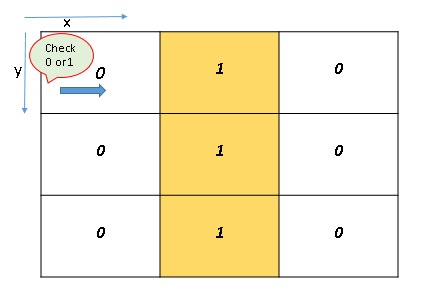
\includegraphics[scale=0.6]{borderfollowingAlgorithm.PNG}\caption{\label{fig:The-simple-}The simple $3\times3$ image demonstrates
the border following algorithm. The yellow pixels are some object
border. The algorithm moves through the pixel grid looking for the
jump in pixel intensities. It memorizes that jump and categorizes
them to respective objects according to their spacial location.}
\par\end{centering}
\end{figure}

The resulting segmented image is shown in figure\ref{fig:Final-segmented-image.}.

\begin{figure}[H]

\begin{centering}
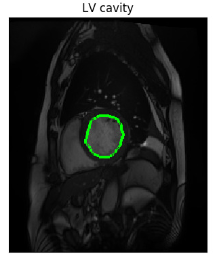
\includegraphics[scale=0.8]{segmented.PNG}\caption{\label{fig:Final-segmented-image.}Final segmented image. The left
ventricle is indicated by green contour. The original image is shown
in figure \ref{fig:On-the-left,}}
\par\end{centering}
\end{figure}


\section{Improvements and Refinements}

initial accuracy , changes made, accuracy increased,

\subsection{First Version}

discuss initial version

\subsection{Second Version}

discuss final version

\section{Final Results}

discuss analyze

\section{Executive Summary}

In this project we used mainly primarily K-Means algorithm inspired
by \cite{lynch2006automatic}. Alongside, a border following algorithm
inspired from \cite{suzuki1985topological} was used to enhance segmentation
results. The preproccessing was done with adaptive smoothing algorithm.
Finally we optimized the performance of our algorithm by repeated
experiments of using the algorithm with different datasets and setting
the parameters to optimal value.

\section{User Guide}

how to use app.

\bibliographystyle{plain}
\bibliography{BibliographyDatabase}


\section*{Appendix A\label{sec:Appendix-A} : Python Libraries Used}
\end{document}
